\chapter{结构体}\label{ch09}

\emph{Long ago, when shepherds wanted to see if two herds of sheep were isomorphic, they would look for an explicit isomorphism}

\begin{flushright}
    ——John C. Baez and James Dolan, “\href{https://arxiv.org/abs/math/9802029}{Categorification}”
\end{flushright}

Rust的结构体,有时也称为\emph{structure},类似于C和C++中的\texttt{struct}类型、Python中的\texttt{class}、JavaScript中的对象。一个结构体把多个不同类型的值组合成单个值,所以你可以将它们作为一个整体进行处理,你也可以读取并且修改结构体的各个组成部分。一个结构体也可以有一些关联的方法来操作它的组成部分。

Rust有三种类型的结构体:\emph{命名字段(name-field)}、\emph{类元组(tuple-like)}、\emph{类单元(unit-like)},它们的区别在于如何引用它们的组成部分:一个命名字段结构体给每一个组件取了一个名字,而类元组结构体用它们出现的顺序来标识它们。类单元结构体没有任何组成部分,它并不常见,但可能比你想象中的更加有用。

在本章中我们将详细解释每一种结构体,并展示它们在内存中的布局。我们将介绍如何给它们添加方法、如何定义可以处理很多不同类型组件的泛型结构体、以及如何让Rust为你的结构体生成通用的trait的实现。

\section{命名字段结构体}

一个命名字段结构体的定义类似于这样:
\begin{minted}{Rust}
    /// 一个8位灰度像素的矩形
    struct GrayscaleMap {
        pixels: Vec<u8>,
        size: (usize, usize)
    }
\end{minted}

这里声明了一个结构体类型\texttt{GrayscaleMap},它有两个字段分别命名为\texttt{pixels}和\texttt{size}。Rust的一个习惯是所有的类型包括结构体,名称中的每一个单词的首字母大写,例如\texttt{GrayscaleMap},这种习惯称为\emph{大驼峰命名法}(或\emph{帕斯卡命名法})。字段和方法名都是小写,用下划线分隔每个单词。这被称为\emph{蛇形命名法}。

你可以用\emph{结构体表达式}构造一个这种类型的值,例如:
\begin{minted}{Rust}
    let width = 1024;
    let height = 576;
    let image = GrayscaleMap {
        pixels: vec![0; width * height],
        size: (width, height)
    };
\end{minted}

结构体表达式以类型名称开始(\texttt{GrayscaleMap}),然后在花括号中列出每一个字段的名称和值。还有一种缩写可以用同名的局部变量来充当字段:
\begin{minted}{Rust}
    fn new_map(size: (usize, usize), pixels: Vec<u8>) -> GrayscaleMap {
        assert_eq!(pixels.len(), size.0 * size.1);
        GrayscaleMap { pixels, size }
    }
\end{minted}

结构体表达式\texttt{GrayscaleMap \{ pixels, size \}}是\texttt{GrayscaleMap \{ pixels: pixels, size: size \}}的缩写。你也可以在使用同名字段缩写的同时使用\texttt{key: value}语法为其它字段赋值。

访问一个结构体的字段需要使用熟悉的\texttt{.}运算符:
\begin{minted}{Rust}
    assert_eq!(image.size, (1024, 476));
    assert_eq!(image.pixels.len(), 1024 * 576);
\end{minted}

和其他item一样,结构体默认是私有的,只在它们声明的模块及其子模块中可见。你可以通过在定义前加\texttt{pub}来让结构体在模块之外也可见。它的每一个字段也是这样,默认也是私有的:
\begin{minted}{Rust}
    /// 一个8位灰度像素的矩形
    pub struct GrayscaleMap {
        pub pixels: Vec<u8>,
        pub size: (usize, usize)
    }
\end{minted}

即使结构体被声明为\texttt{pub},它的字段也可以是私有的:
\begin{minted}{Rust}
    /// 一个8位灰度像素的矩形
    pub struct GrayscaleMap {
        pixels: Vec<u8>,
        size: (usize, usize)
    }
\end{minted}

其他的模块可以使用这个结构体和它的所有公有的关联函数,但不能通过字段名访问私有的字段,也不能通过结构体表达式创建新的\texttt{GrayscaleMap}值。也就是说,创建一个结构体的值要求所有的结构体字段都可见。这也是为什么你不能通过结构体表达式创建新的\texttt{String}或者\texttt{Vec}。这些标准类型都是结构体,但它们的字段全都是私有的。要想创建一个这些类型的值,你必须使用公有的类型关联函数,例如\texttt{Vec::new()}。

在创建一个命名字段结构体值的时候,你可以使用另一个相同类型的结构体来提供你省略的字段的值。在一个结构体表达式中,如果命名字段最后跟着一个\texttt{.. EXPR},那么没有提到的字段将从\texttt{EXPR}中获取值,\texttt{EXPR}必须是另一个相同类型的值。假设我们有一个代表游戏中的怪物的结构体:
\begin{minted}{Rust}
    // 在这个游戏中,连扫帚都是怪物。
    struct Broom {
        name: String,
        height: u32,
        health: u32,
        position: (f32, f32, f32),
        intent: BroomIntent
    }

    /// 一个`Broom`的工作状态有两种可能。
    #[derive(Copy, Clone)]
    enum BroomIntent { FetchWater, DumpWater }
\end{minted}

对程序员来说最好的童话是\emph{魔法师的学徒}:一个魔法师学徒制造了一把能替他工作的扫帚,但工作完成之后却不知道该如何停止它。用斧头把扫帚劈成两半会产生两把扫帚,每个只有一半大小,但仍然像之前一样盲目地继续工作:
\begin{minted}{Rust}
    // 以值接受输入的扫帚,会获取所有权
    fn chop(b: Broom) -> (Broom, Broom) {
        // 用`b`初始化`broom1`的大部分,只修改`height`。因为
        // `String`不是`Copy`,因此`broom1`会获取`b`的name的所有权。
        let mut broom1 = Broom { height: b.height / 2, .. b };

        // 用`broom1`初始化`broom2`的大部分。因为`String`不是
        // `Copy`,所以我们必须显式克隆`name`
        let mut broom2 = Broom { name: broom1.name.clone(), .. broom1 };

        // 给两半分别起不同的名字。
        broom1.name.push_str(" I");
        broom2.name.push_str(" II");
        (broom1, broom2)
    }
\end{minted}

这个定义完成之后,我们可以创建一个扫帚,将它劈成两半,然后我们会得到:
\begin{minted}{Rust}
    let hokey = Broom {
        name: "Hokey".to_string(),
        height: 60,
        width: 100,
        health: 100,
        position: (100.0, 200.0, 0.0),
        intent: BroomIntent::FetchWater
    };

    let (hokey1, hokey2) = chop(hokey);
    assert_eq!(hokey1.name, "Hokey I");
    assert_eq!(hokey1.height, 30);
    assert_eq!(hokey1.health, 100);

    assert_eq!(hokey2.name, "Hokey II");
    assert_eq!(hokey2.height, 30);
    assert_eq!(hokey2.health, 100);
\end{minted}

新的\texttt{hokey1}和\texttt{hokey2}扫帚接收到了新的调整之后的名字,高度减半,其他的值都和原来一样。

\section{类元组结构体}

第二种结构体类型称为\emph{类元组结构体},因为它类似一个元组:
\begin{minted}{Rust}
    struct Bounds(usize, usize);
\end{minted}

你可以像构建元组一样构造一个这种类型的值,除了必须要包含结构体的名字:
\begin{minted}{Rust}
    let image_bounds = Bounds(1024, 768);
\end{minted}

类元组结构体持有的值被称为\emph{元素},就像元组持有的值一样。你可以像访问元组的元素一样访问它们:
\begin{minted}{Rust}
    assert_eq!(image_bounds.0 * image_bounds.1, 786432);
\end{minted}

每一个类元组结构体的元素都可以是公有的或者私有的:
\begin{minted}{Rust}
    pub struct Bounds(pub usize, pub usize);
\end{minted}

表达式\texttt{Bounds(1024, 768)}看起来像一个函数调用,实际上它就是:定义这个类型也会隐式地定义一个同名函数:
\begin{minted}{Rust}
    fn Bounds(elem0: usize, elem1: usize) -> Bounds { ... }
\end{minted}

在底层,命名字段结构体和类元组结构体非常相似。到底用哪一个取决于可读性、二义性和简洁性。如果你将频繁使用\texttt{.}运算符来获取值的组成部分,那么通过名称来标识字段会增强可读性,也更不容易写错。如果你通常用模式匹配来获取元素,那么类元组结构体可以漂亮地完成工作。

类元组结构体常用于\emph{新类型},这种结构体只有单个组件,可以用来获得更严格的类型检查。例如如果你在处理只有ASCII的文本,你可以定义一个这样的新类型:
\begin{minted}{Rust}
    struct Ascii(Vec<u8>);
\end{minted}

使用这种类型表示ASCII字符串比简单的传递\texttt{Vec<u8>}缓冲区好得多,还可以在注释中表明这个类型到底是什么含义。新类型可以帮助Rust捕获其他字节缓冲区被传给期望ASCII文本的函数的错误。我们将在\hyperref[ch22]{第22章}中给出一个使用新类型来实现高效的类型转换的例子。

\section{类单元结构体}

第三种结构体有一点迷惑:它声明了一个没有任何元素的结构体类型:
\begin{minted}{Rust}
    struct Onesuch;
\end{minted}

一个这种类型的值不占用任何内存,类似于单元类型\texttt{()}。Rust不需要考虑怎么在内存中存储类单元结构体,也不需要生成操作它们的代码,因为它可以仅从其类型中得知它可能需要了解的有关值的所有信息。但从逻辑上讲,一个空的结构体和其他的有值的类型没有什么区别——或者更精确地说,一个这样的类型就是一个单独的值:
\begin{minted}{Rust}
    let o = Onesuch;
\end{minted}

当在\nameref{field}一节中介绍\texttt{..}运算符时,你已经遇到过一个类单元结构体了。表达式\texttt{3..5}是结构体值\texttt{Range \{ start: 3, end: 5 \}}的缩写,而表达式\texttt{..}两端都省略的情况下,就是类单元结构体值\texttt{RangeFull}的缩写。

当和trait一起使用时,类单元结构体会变得很有用。我们将在\hyperref[ch11]{第11章}中介绍trait。

\section{结构体布局}

在内存中,命名字段结构体和类元组结构体是同样的东西:一些可能不同类型的值的集合,以一种特殊的方式分布在内存中。例如,我们之前在这一章中定义的这个结构体:
\begin{minted}{Rust}
    struct GrayscaleMap {
        pixels: Vec<u8>,
        size: (usize, usize)
    }
\end{minted}

一个\texttt{GrayscaleMap}按照如\hyperref[f9-1]{图9-1}的布局分布在内存中。

\begin{figure}[htbp]
    \centering
    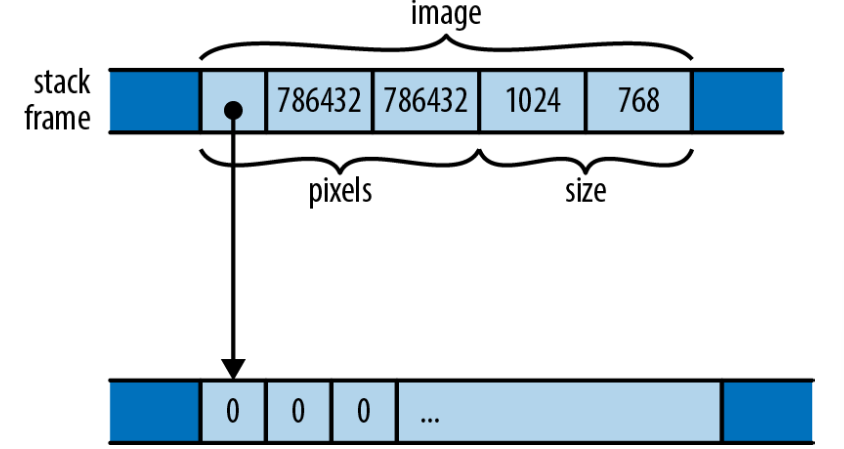
\includegraphics[width=0.8\textwidth]{../img/f9-1.png}
    \caption{一个\texttt{GrayscaleMap}结构体的内存布局}
    \label{f9-1}
\end{figure}

与C和C++不同,Rust对于如何在内存中布局结构体字段或元素没有任何确切的保证,这里的图只是展示了其中一种可能的排列。然而Rust确实保证了直接在结构体的内存块里存储字段的值。JavaScript、Python和Java将会把\texttt{pixels}和\texttt{size}值分别放在它们自己的堆上分配的内存块中,然后让\texttt{GrayscaleMap}的字段指向他们。而Rust会直接把\texttt{pixels}和\texttt{size}嵌入到\texttt{GrayscaleMap}值里。只有\texttt{pixels} vector持有的堆上分配的缓冲区保留着自己的块。

你可以使用\texttt{\#[repr(C)]}属性来要求Rust用一种与C和C++兼容的方式布局结构体。我们将会在\hyperref[ch23]{第23章}中详细介绍这些。

\section{使用\texttt{impl}定义方法}\label{method}

在本书中,我们已经在很多类型的值上调用过方法。我们使用\texttt{v.push(e)}把元素添加进vector,使用\texttt{v.len()}获取它的长度,使用\texttt{r.expect("msg")}检查\texttt{Result}的值是否是错误值,等等。你可以为你自己的结构体类型定义方法。与C++或Java那种直接出现在结构体定义内部的方式不同,Rust的方法在一个单独的\texttt{impl}块中定义。

一个\texttt{impl}块就是一些\texttt{fn}定义的结合,每一个函数都将成为这个结构体的一个方法。例如,这里我们定义了一个公有的结构体\texttt{Queue},然后为它定义了两个公有的方法:\texttt{push}和\texttt{pop}:
\begin{minted}{Rust}
    /// 一个先进先出的字符队列
    pub struct Queue {
        older: Vec<char>,   // 旧的元素,越旧越靠后
        younger: Vec<char>  // 新的元素,越新越靠后
    }

    impl Queue {
        /// 将一个字符添加到队列的尾部。
        pub fn push(&mut self, c: char) {
            self.younger.push(c);
        }

        /// 移出队列最前端的元素,如果有字符被移出就返回`Some(c)`,
        /// 否则如果队列为空就返回`None`。
        pub fn pop(&mut self) -> Option<char> {
            if self.older.is_empty() {
                if self.younger.is_empty() {
                    return None;
                }

                // 将新的元素都移动到旧的元素里,
                // 并且反转顺序。
                use std::mem::swap;
                swap(&mut self.older, &mut self.younger);
                self.older.reverse();
            }

            // 现在旧的元素保证不为空。Vec的pop方法
            // 已经返回了一个Option,因此不用再处理
            self.older.pop()
        }
    }
\end{minted}

在\emph{impl}块中定义的函数被称为\emph{关联函数},因为它们被关联到特定的类型。与之相反的是\emph{自由函数},也就是不在\texttt{impl}块中定义的函数。

Rust将调用方法的值作为第一个参数传给方法,它的参数名必须是\texttt{self}。因为\texttt{self}的类型很明显是\texttt{impl}块外面的结构体类型,或者是其引用,所以Rust允许你省略类型,用\texttt{self}、\texttt{\&self}、\texttt{\&mut self}分别作为\texttt{self: Queue}、\texttt{self: \&Queue}、\texttt{self: \&mut Queue}的缩写。如果你喜欢的话也可以使用非缩写的形式,但几乎所有的Rust代码都是用缩写形式。

在我们的示例中,\texttt{push}和\texttt{pop}方法中通过\texttt{self.older}和\texttt{self.younger}引用了\texttt{Queue}的字段。与C++或Java中“this”对象的成员直接在方法内可见不同,Rust方法中必须显式使用\texttt{self}来引用字段,这和Python方法中\texttt{self}的用法、JavaScript方法中\texttt{this}的用法类似。

因为\texttt{push}和\texttt{pop}需要修改\texttt{Queue},所以它们都以\texttt{\&mut self}传参。然而,当你调用这两个方法时,你不需要手动借用可变引用,普通的方法调用语法会自动进行隐式转换。因此有了这些定义之后,你可以像这样使用\texttt{Queue}:
\begin{minted}{Rust}
    let mut q = Queue { older: Vec::new(), younger: Vec::new() };

    q.push('0');
    q.push('1');
    assert_eq!(q.pop(), Some('0'));

    q.push('=');
    assert_eq!(q.pop(), Some('1'));
    assert_eq!(q.pop(), Some('='));
    assert_eq!(q.pop(), None);
\end{minted}

为了满足\texttt{push}方法的\texttt{self}参数要求,直接写\texttt{q.push(...)}会借用\texttt{q}的可变引用,就像你写了\\
\texttt{(\&mut q).push(...)}一样。

如果一个方法不需要修改\texttt{self},那么你可以以共享引用获取参数。例如:
\begin{minted}{Rust}
    impl Queue {
        pub fn is_empty(&self) -> bool {
            self.older.is_empty() && self.younger.is_empty()
        }
    }
\end{minted}

方法调用表达式知道要借用哪一种引用:
\begin{minted}{Rust}
    assert!(q.is_empty());
    q.push('☉');
    assert!(!q.is_empty());
\end{minted}

或者,如果一个方法想获取\texttt{self}的所有权,它可以以值传递\texttt{self}:
\begin{minted}{Rust}
    impl Queue {
        pub fn split(self) -> (Vec<char>, Vec<char>) {
            (self.older, self.younger)
        }
    }
\end{minted}

调用这个\texttt{split}方法看起来和调用其他方法一样:
\begin{minted}{Rust}
    let mut q = Queue { older: Vec::new(), younger: Vec::new() };

    q.push('P');
    q.push('D');
    assert_eq!(q.pop(), Some('P'));
    q.push('X');

    let (older, younger) = q.split();
    // q现在是未初始化状态
    assert_eq!(older, vec!['D']);
    assert_eq!(younger, vec!['X']);
\end{minted}

但是注意,因为\texttt{split}以值获取\texttt{self},这会把\texttt{q}中的\texttt{Queue}值\emph{移动}走,导致\texttt{q}变为未初始化。因为\texttt{split}的\texttt{self}现在拥有了这个队列,因此它可以把两个单独的vector移动出来并返回给调用者。

有时,像这样以值传递\texttt{self},或者以引用传递都不能满足我们的需求,因此Rust还允许你通过智能指针类型传递\texttt{self}。

\subsection{以\texttt{Box}、\texttt{Rc}、\texttt{Arc}传递\texttt{Self}}

一个方法的\texttt{self}参数还可以是\texttt{Box<Self>}、\texttt{Rc<Self>}、\texttt{Arc<Self>}。这些方法只能在相应指针类型上调用。调用这些方法会传递指针的所有权。

你通常不需要这么做。一个以引用传递\texttt{self}的方法可以在任何智能指针类型上正常调用:
\begin{minted}{Rust}
    let mut bq = Box::new(Queue::new());

    // `Queue::push`接受一个`&mut Queue`,但`bq`是`Box<Queue>`。
    // 这没有问题:Rust在调用期间从`Box`借用了一个`&mut Queue`
    bq.push('■');
\end{minted}

对于方法调用和字段访问,Rust自动从智能指针类型例如\texttt{Box}、\texttt{Rc}和\texttt{Arc}借用一个引用,因此\texttt{\&self}和\texttt{\&mut self}通常总是正确的方法签名,再加上偶尔用到的\texttt{self}。

但如果这个方法的意图涉及管理指针的所有权呢?假设我们有一个像这样的节点组成的树,类似某种彻底简化的XML:
\begin{minted}{Rust}
    use std::rc::Rc;

    struct Node {
        tag: String,
        children: Vec<Rc<Node>>
    }

    impl Node {
        fn new(tag: &str) -> Node {
            Node {
                tag: tag.to_string(),
                children: vec![],
            }
        }
    }
\end{minted}

每一个节点都有一个tag来指示它是什么类型的节点,还有一个子节点的vector通过引用计数指针来允许共享,并让生命周期变得更灵活。

通常我们会实现一个方法让它向自己的列表中添加一个子节点,但现在让我们把角色颠倒过来,给\texttt{Node}实现一个把它自己添加到别的\texttt{Node}的子节点中的方法。我们可以写:
\begin{minted}{Rust}
    impl Node {
        fn append(self, parent: &mut Node) {
            parent.children.push(Rc::new(self));
        }
    }
\end{minted}

但这个方法并不能让人满意。这个方法调用了\texttt{Rc::new}来分配新的堆空间并且把\texttt{self}移动进去,但如果调用者已经有了一个\texttt{Rc<Node>},这些操作就都不是必须的:我们应该只递增引用计数然后把指针加到vector里。\texttt{Rc}的全部意义不就是实现共享吗?

我们可以这样写:
\begin{minted}{Rust}
    impl Node {
        fn append_to(self: Rc<Self>, parent: &mut Node) {
            parent.children.push(self);
        }
    }
\end{minted}

如果调用者已经是\texttt{Rc<Node>}类型,那它可以直接调用\texttt{append\_to},以值传递\texttt{Rc}:
\begin{minted}{Rust}
    let shared_node = Rc::new(Node::new("first"));
    shared_node.append_to(&mut parent);
\end{minted}

这会把\texttt{shared\_node}的所有权传递给方法:引用计数不会发生变化,也不会有新的内存分配。

如果调用者需要保留节点的指针以便之后使用,它可以首先克隆\texttt{Rc}再调用:
\begin{minted}{Rust}
    shared_node.clone().append_to(&mut parent);
\end{minted}

克隆\texttt{Rc}只会递增引用计数,没有堆分配或者拷贝。但当调用返回时\texttt{shared\_node}和\texttt{parent}\\
的子节点的vector现在指向同一个\texttt{Node}。

最后,如果调用者现在拥有一个\texttt{Node},那么它必须先创建一个\texttt{Rc}再调用方法:
\begin{minted}{Rust}
    let owned = Node::new("owned directly");
    Rc::new(owned).append_to(&mut parent);
\end{minted}

把\texttt{append\_to}方法的签名设为\texttt{Rc<Self>}可以让调用者知道\texttt{Node}的需求。然后调用者可以用最小化内存分配和引用计数调整的方式来调用:
\begin{itemize}
    \item 如果可以传递\texttt{Rc}的所有权,就直接在指针上调用。
    \item 如果需要保留\texttt{Rc}的所有权,就递增引用计数后再调用。
    \item 如果只拥有\texttt{Node},那么必须先调用\texttt{Rc::new}来分配堆空间然后把\texttt{Node}移动进去。因为\texttt{parent}必须通过\texttt{Rc<Node>}指针引用它的子节点,所以这一步最终肯定是必须的。
\end{itemize}

再重复一遍,对于大多数方法,\texttt{\&self}、\texttt{\&mut self}、和\texttt{self}(以值传参)就能满足你的需求。但如果一个方法的目的是影响值的所有权,使用其他指针类型的\texttt{self}可能是正确的选择。

\subsection{类型关联函数}
\texttt{impl}块里定义的函数也可以没有\texttt{self}参数。这些参数仍然和类型关联,因为它们也是在\texttt{impl}块中定义的。但它们不是方法,因为它们没有\texttt{self}参数。为了将它们和方法区别开来,我们称它们为\emph{类型关联函数}。

它们通常用于提供构造函数,例如:
\begin{minted}{Rust}
    impl Queue {
        pub fn new() -> Queue {
            Queue { older: Vec::new(), younger: Vec::new() }
        }
    }
\end{minted}

为了使用这个函数,我们通过\texttt{Queue::new}来引用它:类型名+双冒号+函数名。现在我们的示例代码变得更加简洁:
\begin{minted}{Rust}
    let mut q = Queue::new();

    q.push('*');
    ...
\end{minted}

Rust的传统是构造函数都叫\texttt{new},我们已经见过了\texttt{Vec::new}、\texttt{Box::new}、\texttt{HashMap::new},等等。但\texttt{new}这个名字本身并没有什么特殊的地方。它并不是关键字,而且一个类型经常还有其他名字的关联函数作为构造函数,例如\texttt{Vec::with\_capacity}。

尽管一个类型可以有很多个分开的\texttt{impl}块,但它们必须在定义类型的那个crate中。然而,Rust确实允许你将自己定义的方法附加到其他类型,我们将在\hyperref[ch11]{第11章}介绍怎么做到这一点。

如果你习惯写C++或Java,你可能会觉得将类型的方法和定义分离开来很奇怪,但这么做确实有以下优势:
\begin{itemize}
    \item 你总是能很容易的找到一个类型的数据成员。在很大的C++类定义中,你可能需要浏览几百行成员成员函数的定义来确保你没有遗漏数据成员。而在Rust中,所有数据成员都在一个地方。
    \item 尽管我们可以很容易想象把方法定义添加到命名字段结构体的定义中,但类元组结构体和类单元结构体却不是这样。将方法拿出来放在一个\texttt{impl}块中可以让这三种结构体共用唯一一种语法。事实上,Rust还使用这套语法为不是结构体的类型定义方法,例如\texttt{enum}结构体和基本类型例如\texttt{i32}。(任何类型都可以有方法的事实是Rust中不使用术语\emph{对象},而是更喜欢把一切称为\emph{值}的原因之一。)
    \item 同样的\texttt{impl}语法还可以很容易地用于实现trait,我们将在\hyperref[ch11]{第11章}中介绍。
\end{itemize}

\section{关联常量}
Rust的类型系统还采用了C\#和Java等语言中的一个特性,就是关联到类型而不是关联到类型实例的值。在Rust中,它们被称为\emph{关联常量}。

正如它的名字一样,关联常量是常量值。它们通常用来表示某一个类型中使用最广泛的值。例如,你可以定义一个二维的向量用于线性代数,并为它定义一个关联的单位向量:
\begin{minted}{Rust}
    pub struct Vector2 {
        x: f32,
        y: f32,
    }

    impl Vector2 {
        const ZERO: Vector2 = Vector2 { x: 0.0, y: 0.0 };
        const UNIT: Vector2 = Vector2 { x: 1.0, y: 0.0 };
    }
\end{minted}

这些值被关联到类型本身,你可以在不创建\texttt{Vector2}的实例的情况下使用它们。和类型关联方法一样,引用它们的方法是类型的名称再加上它们的名称:
\begin{minted}{Rust}
    let scaled = Vector2::UNIT.scaled_by(2.0);
\end{minted}

关联常量的类型并不一定必须是它关联的类型,我们可以使用这个特性来给类型添加ID或者名称。例如,如果有几个和\texttt{Vector2}很像的类型需要写入到文件里,然后加载到内存中,那么关联常量可以为写入的数据添加名称或数字ID,这样之后可以据此辨识出类型:
\begin{minted}{Rust}
    impl Vector2 {
        const NAME: &'static str = "Vector2";
        const ID: u32 = 18;
    }
\end{minted}

\section{泛型结构体}\label{GenStruct}

我们之前的\texttt{Queue}定义并不能令人满意:它被用来存储字符,但它却没有任何和字符相关的方法。如果我们要定义另一个存储\texttt{String}值的结构体,那么除了\texttt{char}要换成\texttt{String}之外,剩下的代码完全相同。重复定义将会浪费时间。

幸运的是,Rust的结构体可以是\emph{泛型}的,这意味着它们的定义只是一个模板,你可以把任何类型塞进去。例如,这里有一个可以存储任何类型的值的\texttt{Queue}的定义:
\begin{minted}{Rust}
    pub struct Queue<T> {
        older: Vec<T>,
        younger: Vec<T>
    }
\end{minted}

你可以将\texttt{Queue<T>}中的\texttt{<T>}读作“对于任意类型\texttt{T}”。因此这个定义读作“对于任意类型\texttt{T},一个\texttt{Queue<T>}有两个\texttt{Vec<T>}类型的字段。”例如,在\texttt{Queue<String>}中,\texttt{T}是\texttt{String},所以\texttt{older}和\texttt{younger}的类型都是\texttt{Vec<String>}。在\texttt{Queue<char>}中\texttt{T}是\texttt{char},我们就得到了一个和一开始的\texttt{char}类型特定的定义完全相同的结构体。事实上,\texttt{Vec}本身就是一个用这种方式定义的泛型结构体。

在泛型结构体的定义中,<尖括号>里的类型名被称为\emph{类型参数}。一个泛型结构体的\texttt{impl}块看起来像这样:
\begin{minted}{Rust}
    impl<T> Queue<T> {
        pub fn new() -> Queue<T> {
            Queue { older: Vec::new(), younger: Vec::new() }
        }

        pub fn push(&mut self, t: T) {
            self.younger.push(t);
        }

        pub fn is_empty(&self) -> bool {
            self.older.is_empty() && self.younger.is_empty()
        }

        ...
    }
\end{minted}

你可以将\texttt{impl<T> Queue<T>}这一行读作“对于任意类型\texttt{T},有一些\texttt{Queue<T>}可用的关联方法”。然后,你可以在关联函数的定义中将类型参数\texttt{T}用作一个类型。

这种语法看起来好像有些重复,但\texttt{impl<T>}能更清晰地表达出\texttt{impl}块覆盖了任意的类型\texttt{T},这能将它和为特定种类的\texttt{Queue}编写的\texttt{impl}块区分开来,例如:
\begin{minted}{Rust}
    impl Queue<f64> {
        fn sum(&self) -> f64 {
            ...
        }
    }
\end{minted}

这个\texttt{impl}块头读作“这里有一些\texttt{Queue<f64>}特定的关联方法”。这样就给\texttt{Queue<f64>}添加了一个\texttt{sum}方法,而其它种类的\texttt{Queue}并没有这个方法。

我们已经在之前的代码中使用过Rust的\texttt{self}参数的缩写形式。这里\texttt{Queue<T>}如果写出类型显得有些啰嗦。作为另一种缩写,每一个\texttt{impl}块,不管是不是泛型的,都定义了特殊的类型参数\texttt{Self}(注意\texttt{大驼峰}风格的名称)来表示我们要添加方法的类型。在之前的代码中,\texttt{Self}将是\texttt{Queue<T>},因此我们可以进一步简化\texttt{Queue::new}的定义:
\begin{minted}{Rust}
    pub fn new() -> Self {
        Queue { older: Vec::new(), younger: Vec::new() }
    }
\end{minted}

你可能已经注意到了,在\texttt{new}的函数体内,我们不需要在构造表达式中写出类型参数,简单地写\texttt{Queue \{ ... \}}就足够了。这是因为Rust的类型推导发挥了作用:因为函数的返回值类型只能有一种可能,就是\texttt{Queue<T>},所以Rust会自动为我们提供参数。然而,你必须总是在函数签名和类型定义中指明类型参数。Rust不会推断它们,相反,它将这些已知的类型作为基础来推断那些函数体内的类型。

\texttt{Self}也可以用于这种方式:我们可以写\texttt{Self \{ ... \}}。你觉得哪种形式更容易理解就可以用哪种。

对于关联函数的调用,你可以显式地使用\texttt{::<>(涡轮鱼)}注解来提供类型参数:
\begin{minted}{Rust}
    let mut q = Queue::<char>::new();
\end{minted}

但在实践中,通常可以让Rust自动帮你推断类型:
\begin{minted}{Rust}
    let mut q = Queue::new();
    let mut r = Queue::new();

    q.push("CAD");      // 显然是Queue<&'static str>
    r.push(0.74);       // 显然是Queue<f64>

    q.push("BTC");      // 比特币/USD,2019年6月 
    r.push(13764.0);    
\end{minted}

事实上,这正是整本书中我们使用\texttt{Vec}的方式。

并不只有结构体可以是泛型的。枚举也可以有类型参数,语法也非常的相似。我们将在\nameref{enum}一节中详细介绍。

\section{有生命周期参数的结构体}

正如我们在\nameref{refstruct}一节中讨论过的一样,如果一个结构体类型中包含引用,你必须指明那些引用的生命周期。例如,这里有一个存储切片中最大和最小元素的引用的结构体:
\begin{minted}{Rust}
    struct Extrema<'elt> {
        greatest: &'elt i32,
        least: &'elt i32
    }
\end{minted}

之前,我们建议你将类似\texttt{struct Queue<T>}的声明看作是对于任意类型\texttt{T},你都可以构建一个\texttt{Queue<T>}来存储该类型。类似的,你可以将\texttt{struct Extrema<'elt>}看作对于任意生命周期\texttt{'elt},你都可以构建一个\texttt{Extrema<'elt>}来存储生命周期为\texttt{'elt}的引用。

这里有一个函数来扫描一个切片并返回一个指向其中元素的\texttt{Extrema}值:
\begin{minted}{Rust}
    fn find_extrema<'s>(slice: &'s [i32]) -> Extrema<'s> {
        let mut greatest = &slice[0];
        let mut least = &slice[0];

        for i in 1..slice.len() {
            if slice[i] < *least    { least     = &slice[i]; }
            if slice[i] > *greatest { greatest  = &slice[i]; }
        }
        Extrema { greatest, least }
    }
\end{minted}

这里,\texttt{find\_extrema}借用了\texttt{slice}的元素。因为\texttt{slice}的生命周期是\texttt{'s},所以我们返回的\texttt{Extrema}结构体中的引用的生命周期也是\texttt{'s}。Rust总是会为调用推断生命周期参数,因此调用\texttt{find\_extrema}并不需要提到它们:
\begin{minted}{Rust}
    let a = [0, -3, 0, 15, 48];
    let e = find_extrema(&a);
    assert_eq!(*e.least, -3);
    assert_eq!(*e.greatest, 48);
\end{minted}

因为返回值和参数使用相同的生命周期非常常见,所以当只有一种可能时Rust允许我们省略生命周期。我们还可以在不改变含义的情况下将\texttt{find\_extrema}的签名写成这样:
\begin{minted}{Rust}
    fn find_extrema(slice: &[i32]) -> Extrema {
        ...
    }
\end{minted}

诚然,我们也\emph{可能}是想返回\texttt{Extrema<'static>},但这并不是通常的情况。Rust只为通常的情况提供了一个缩写。

\section{为结构体类型派生常见的trait}

可以非常简单地定义一个结构体:
\begin{minted}{Rust}
    struct Point {
        x: f64,
        y: f64
    }
\end{minted}

然而,如果你真的开始使用这个\texttt{Point}类型,你将很快发现它使用起来很痛苦。按照上面的写法,\texttt{Point}既不能拷贝也不能克隆。你不能用\texttt{println!("\{:?\}", point);}打印它,它也不支持\texttt{==}和\texttt{!=}运算符。

在Rust中这些特性都有一个名字——\texttt{Copy}、\texttt{Clone}、\texttt{Debug}、\texttt{PartialEq}。它们被称为\emph{trait}。在\hyperref[ch11]{第11章}中,我们将展示如何为你自己的结构体手动实现trait。但这个例子中出现的标准trait,以及其它一些trait,你不需要手动实现它们,除非你想要一些自定义行为。Rust可以自动为你实现它们。只需要为结构体添加\texttt{\#[derive]}属性:
\begin{minted}{Rust}
    #[derive(Copy, Clone, Debug, PartialEq)]
    struct Point {
        x: f64,
        y: f64
    }
\end{minted}

这些trait中的任何一个都可以自动实现,前提是这个结构体的所有字段都实现了那个trait。我们可以要求Rust为\texttt{Point}派生\texttt{PartialEq},是因为它的两个字段都是\texttt{f64}类型,这个类型已经实现了\texttt{PartialEq}。

Rust还可以派生\texttt{PartialOrd},它可以支持比较运算符\texttt{<}、\texttt{>}、\texttt{<=}和\texttt{>=}。我们没有这么做,是因为比较两个点来判断其中一个是否“小于”另一个是一件很奇怪的事。因此我们选择让\texttt{Point}值不支持那些比较运算符。像这样的情况也是Rust让我们自己写\texttt{\#[derive]}属性而不是直接自动派生所有可用的trait的原因之一。另一个原因是实现一个trait将自动变为公有的特性。因此可复制性、可克隆性等都将是结构体公共API的一部分,应该慎重选择。

我们将在\hyperref[ch13]{第13章}详细介绍Rust的标准trait并解释哪些可以用\texttt{\#[derive]}自动实现。

\section{内部可变性}\label{intermut}

可变性和其他东西一样:如果限制太过宽松就会导致问题,但你又总是希望它能放宽一点。例如,假设你的蜘蛛机器人控制系统是一个中心化的结构体\texttt{SpiderRobot},这个结构体里包含设置和I/O处理。当机器人启动时它的值就被初始化,并且永远不会改变:
\begin{minted}{Rust}
    pub struct SpiderRobot {
        species: String,
        web_enabled: bool,
        leg_devices: [fd::FileDesc; 8],
        ...
    }
\end{minted}

机器人的每一个主要系统都由一个不同的结构体处理,这些结构体都有一个指向那个\texttt{SpiderRobot}值的指针:
\begin{minted}{Rust}
    use std::rc::Rc;

    pub struct SpiderSenses {
        robot: Rc<SpiderRobot>, // <-- 指向设置和I/O的指针
        eyes: [Camera; 32],
        motion: Accelerometer,
        ...
    }
\end{minted}

控制织网、捕食、毒液流动等的结构体都有一个\texttt{Rc<SpiderRobot>}智能指针。回顾一下,\texttt{Rc}代表\hyperref[rc]{引用计数},、\texttt{Rc}中的值总是共享的因此总是不可变的。

现在假设你想使用标准的\texttt{File}类型给\texttt{SpiderRobot}结构体添加一点日志功能。那么就会有一个问题:\texttt{File}值必须是\texttt{mut}的。所有写入它的函数都需要\texttt{mut}引用。

这种情况经常出现。我们需要的是一个不可变(\texttt{SpiderRobot}结构体)的值内有一小部分数据可变(一个\texttt{File})。这被称为\emph{内部可变性}。Rust为此提供了几种方式,这一节中我们将讨论最直观的两种类型:
\texttt{Cell<T>}和\texttt{RefCell<T>},这两个类型都在\texttt{std::cell}模块中。

\texttt{Cell<T>}结构体只包含单个私有的类型\texttt{T}的值。\texttt{Cell}唯一特殊的地方是即使你没有对\texttt{Cell}自身的\texttt{mut}访问权限,也可以访问和修改它里面的字段值:

\codeentry{Cell:new(value)}
\hangparagraph{创建一个新的\texttt{Cell},将给定的\texttt{value}移动进去。}

\codeentry{cell.get()}
\hangparagraph{返回一个\texttt{cell}中值的拷贝}

\codeentry{cell.set(value)}
\hangparagraph{将给定的值\texttt{value}存储在\texttt{cell}中,丢弃掉之前存储的值。这个方法以非\texttt{mut}引用获取\texttt{self}参数:}
\begin{minted}{Rust}
    fn set(&self, value: T) // 注意:不是`&mut self`
\end{minted}
\hangparagraph{显然,这和普通的\texttt{set}方法不同。到目前为止,Rust告诉我们如果想要修改数据就需要\texttt{mut}访问权限。但同样的道理,这一处不同的细节就是\texttt{Cell}全部的精髓。它们是一种安全地扭曲不可变性规则的方式——既不多、也不少。}

\texttt{Cell}还可以有一些其他的方法,你可以在\href{https://doc.rust-lang.org/std/cell/struct.Cell.html}{它的文档}中查阅。

如果你想给你的\texttt{SpiderRobot}添加一个简单的计数器,那么使用\texttt{Cell}将会很方便。你可以写:
\begin{minted}{Rust}
    use std::cell::Cell;

    pub struct SpiderRobot {
        ...
        hardware_error_count: Cell<u32>,
        ...
    }
\end{minted}

即使是\texttt{SpiderRobot}的非\texttt{mut}方法也可以使用\texttt{.get()}和\texttt{.set()}来访问\texttt{u32}:
\begin{minted}{Rust}
    impl SpiderRobot {
        /// 错误计数加一
        pub fn add_hardware_error(&self) {
            let n = self.hardware_error_count.get();
            self.hardware_error_count.set(n + 1);
        }

        /// 如果有硬件错误的话返回真
        pub fn has_hardware_errors(&self) -> bool {
            self.hardware_error_count.get() > 0
        }
    }
\end{minted}

这非常简单,但并不能解决我们的日志问题。\texttt{Cell}\emph{不能}让你调用内含值的\texttt{mut}方法,因为\texttt{.get()}方法返回的是单元里值的拷贝,所以它只能用于实现了\hyperref[copy]{\texttt{Copy} trait}的类型。为了实现日志功能,我们需要一个可变的\texttt{File},而\hyperref[file]{\texttt{File}}不可拷贝。

这个例子中正确的工具是\texttt{RefCell}。类似于\texttt{Cell<T>},\texttt{RefCell<T>}也是一个包含单个\texttt{T}类型的值的泛型类型。和\texttt{Cell}不同的是,\texttt{RefCell}支持借用内部的\texttt{T}类型的值:

\codeentry{RefCell::new(value)}
\hangparagraph{创建一个新的\texttt{RefCell},把\texttt{value}移动进去。}

\codeentry{ref\_cell.borrow()}
\hangparagraph{返回一个\texttt{Ref<T>},它本质上是\texttt{ref\_cell}里存储的值的一个共享引用。}
\hangparagraph{如果里面的值已经有可变借用了,这个方法会panic。}

\codeentry{ref\_cell.borrow\_mut()}
\hangparagraph{返回一个\texttt{RefMut<T>},它本质上是\texttt{ref\_cell}里存储的值的一个可变引用。}
\hangparagraph{如果里面的值已经被借用了,这个方法会panic。}

\codeentry{ref\_cell.try\_borrow(), ref\_cell.try\_borrow\_mut()}
\hangparagraph{与\texttt{borrow()}和\texttt{borrow\_mut()}的功能一样,但返回一个\texttt{Result}。当值已经有可变借用/被借用时,它们不panic,而是返回一个\texttt{Err}值。}

同样的,\texttt{RefCell}还有一些其它方法,你可以在\href{https://doc.rust-lang.org/std/cell/struct.RefCell.html}{它的文档}中查阅。

只有当你尝试打破Rust中\texttt{mut}引用必须是独占引用的规则时这两个方法才会panic。例如,这样将会panic:
\begin{minted}{Rust}
    use std::cell::RefCell;

    let ref_cell: RefCell<String> = RefCell::new("hello".to_string());

    let r = ref_cell.borrow();  // ok,返回一个Ref<String>
    let count = r.len();        // ok, 返回"hello".len()
    assert_eq!(count, 5);       

    let mut w = ref_cell.borrow_mut(); // panic:已经被借用了
    w.push_str(" world");
\end{minted}

为了避免panic,你可以把这两个借用放进单独的块里。这样的话,\texttt{r}会在你尝试借用\texttt{w}之前被drop。

这和普通引用的工作方式很像。唯一的不同在于普通的情况下,当你尝试借用一个变量的引用,Rust会在\emph{编译期}确保你必须安全地使用引用。如果检查失败了,你会得到一个编译期错误。\texttt{RefCell}使用运行时检查来执行同样的规则。如果你尝试打破规则,你会得到一个panic(或者使用\texttt{try\_borrow}和\texttt{try\_borrow\_mut}时会得到一个\texttt{Err})。

现在我们已经准备好用\texttt{RefCell}来完善我们的\texttt{SpiderRobot}了:
\begin{minted}{Rust}
    pub struct SpiderRobot {
        ...
        log_file: RefCell<File>,
        ...
    }

    impl SpiderRobot {
        /// 向日志文件中写入一行。
        pub fn log(&self, message: &str) {
            let mut file = self.log_file.borrow_mut();
            // `writeln!`和`println!`很像,
            // 但会把字符串写入到给定的文件中。
            writeln!(file, "{}", message).unwrap();
        }
    }
\end{minted}

变量\texttt{file}的类型是\texttt{RefMut<File>}。它的使用方式就像\texttt{File}的可变引用一样。有关写入文件的细节,见\hyperref[ch18]{第18章}。

Cell很容易使用。虽然必须调用\texttt{.get()}和\texttt{.set()}或者\texttt{.borrow()}和\texttt{.borrow\_mut()}有点麻烦,但那只是我们扭曲可变性规则的代价。还有一些不是很明显但却更严重的问题:Cell——和任何包含了它们的类型——都不是线程安全的。因此Rust\hyperref[threadsafe]{不允许}多个线程直接访问它们。我们将在\hyperref[ch19]{第19章}中讨论到\nameref{mutex}、\nameref{atomic}和\nameref{globalvar}时介绍多线程中的内部可变性。

不管一个结构体有命名字段还是类元组结构体,它都是一些其他值的聚合体:如果我有一个\texttt{SpiderSenses}结构体,那么我就有一个指向共享的\texttt{SpiderRobot}结构体的\texttt{Rc}指针、同时还有了eyes、accelerometer等等。因此结构体的本质是单词“和(and)”:我有一个X\emph{和(and)}一个Y。但是否有另一种类型用于单词“或(or)”呢?换句话说,当你有了一个这种类型的值时,你有了一个X\emph{或(or)}一个Y?这样的类型太有用了以至于它们在Rust中无处不在,它们就是我们下一章要讨论的主题。
